
\section{Proposal}
\label{sec:prop}
% Proposal:
%  - retomar problema {iot, sec, ND};
%  - objetivo;
%  - soluções {MINAS, paralelismo, distribuído, ~~py-kafka, flink,~~ mpi}
%  - propor uma solução

% \begin{highlight}
% A expansão do IoT na industria e vida diária\\
% leva a maior incidência de intrusão e subversão\\
% portanto são necessários sistemas de detectão de intrusão\\
% eficases (boa acuracia) e eficientes (baixa latência)\\
% portanto propôen-se\\
% um NIDS que utiliza algoritmo de detecção de novidades (para acurárcia)\\
% implementado de maneira distruída na borda e nuvem (para latência).\\
% \end{highlight}

%Amid of \iot expansion in multiple fields, from industry to daily life, the constant threat of intrusion
% , subversion (overthrow), denial of service (or any other unexpected detrimental behavior)
% by any component of a system or external actors is a prospect looming over many systems administrators and for that reason
% Thus,  new network surveillance tools are needed, especially effective (accurate) and efficient (fast reaction and good throughput) \nids.
% Following that reasoning, new \nids and other autonomous and analytic system
% surveillance tools are being proposed, many employing techniques such as Anomaly
% and Novelty Detection.
% These tools require the network packet traffic to be constantly analysed,

% Este apresenta uma proposta de implementação distribuida do MINAS que segue as diretrizes da arquitetura IDSA-IoT, atendendo aos seguintes requisitos:
% (i) a etapa de classificação de vários fluxos deve ocorrer em paralelo, sendo processada em diversos locais físicos da arquitetura 
% (ii) a etapa de detecção de novidades (evolução do modelo) deve ocorrer em paralelo, sendo processada em diversos locais físicos da arquitetura 
% (iii)  as duas etapas anteriores, por sua vez também deverão ser executadas paralelamente, podendo ocorrer em partes distintas do sistema
% (iv) possa ser implementada em dispositivos com recursos limitados 

In this work we investigate the use of the novelty detection techniques and strategies,
presented by the MINAS algorithm~\cite{MINAS} and the IDSA-IoT architecture~\cite{Cassales2019a},
by implementation and evaluation of a parallel and distributed descendant of those two works
we named \mfog.
However, given the distributed nature and the typical use of 
low-end devices in envisioned and currently deployed IoT scenarios,  
new constraints apply:
\begin{enumerate*}[label=(\emph{\roman*})]
    \item the classification phase of the algorithm must occur in parallel,
    at different spots at the same time;
    \item the novelty detection phase, which provides the model evolution,
    must also occur in parallel, at different spots;
    \item both phases must also operate in parallel,
    possibly at different places/nodes of the system;
    \item the algorithm complexity must allow it to be processed by modest computer devices.
\end{enumerate*}


% \todo{Relembrar ids-iot, fase offline e online}

Thus we propose a \nids using MINAS \cite{Faria2016minas}
% (a Novelty Detection algorithm)
to effectively identify previous and new intrusion threats,
implemented by following the  architecture \cite{Cassales2019a} using parallel and distributed techniques leveraging
edge and cloud for efficient computing.

% \todo{[start] intro/related?}
\nids 
monitor the packet network traffic, aggregate into flow descriptors and
% aggregated into flow descriptors and further processed in a classification
analyze to identify any intrusion or misbehavior.
% using methods such as classification and Novelty Detection
% This requirement in turn, requesting more computing power at the edge.
% While requesting more computing power in a cloud environment is trivial and
% inexpensive, the same cannot be said 
However, this problem requires both fast and accurate response \cite{DaCosta2019a}:
fast response is needed to have a proper reaction before harm can be cast
to the network and to cope with the traffic without imposing loss or delay
in the \nids or observed network;
accurate response is required as to not misidentify harmless with harmful and vice-versa,
especially the case of false positive that leads to false alarms.
To achieve those goals we leverage fog computing.

% \hl{intro/related?}

In common \iot scenarios, data is captured by small devices and sent to the
cloud for any compute or storage tasks, but this is not feasible in our
\nids scenario. Even though we also capture data produced in the edge,
sending this data to the cloud would in the worst case double the
internet communication requirements of the overall system.
Fog computing infrastructure aims to offload
computing resources from cloud providers by placing edge
devices closer to end-users and/or data sources.
But two MINAS steps limit this fog offload,
the processing intensive novelty detection and,
long term model storage and distribution of the internal model.
Those steps surpass the capabilities of common fog hardware and
therefore need to be at least shared to a cloud where such
requirements are easy and cheap to fulfill.
% \todo{[end] intro/related?}

In our proposed \nids, fog and cloud computing resources are
employed as to minimize the time elapsed between a flow descriptor
ingestion and intrusion alarm, allocating the 
classification step of MINAS in a MPI cluster running multiple
classifier instances.
After the initial classification, the resulting label can be used immediately,
but if the sample is labeled as \emph{unknown}, this sample must be stored
and the novelty detection step will be triggered, and those steps require more resources
and thus are divided in fog and cloud.

% Therefore, our objective is a Distributed novelty detection in streams using limited hardware.
% Previous attempts to attain the objective of distributed fast


\begin{algorithm}[htb]
% {\scriptsize
% \begin{multicols}{2}
    % \SetAlgoVlined
    \SetKwProg{Function}{Function}{:}{}
    \SetKwFor{With}{with}{}{}
    \SetKw{continue}{continue}
    % 
    \SetKwData{MEPC}{MEPC}
    \SetKwData{NF}{NF}
    \SetKwData{mpiSize}{mpiSize}
    \SetKwData{mpiRank}{mpiRank}
    \SetKwData{EndOfStream}{EndOfStream}
    % 
    \SetKwInOut{KwParams}{Parameters}
    \KwParams{mpiNodeRank as \mpiRank}
    % 
    \SetKwFunction{Mfog}{Mfog}
    \SetKwFunction{Sampler}{Sampler}
    \SetKwFunction{Classifier}{Classifier}
    \SetKwFunction{Detector}{Detector}
    \SetKwFunction{modelReceiver}{modelReceiver}
    % 
    \SetKwFunction{typeOf}{typeOf}
    % 
    \SetKwFunction{Thread}{Thread}
    \SetKwFunction{Lock}{Lock}
    \SetKwFunction{readLock}{readLock}
    \SetKwFunction{writeLock}{writeLock}
    % 
    \SetKwFunction{receive}{receive}
    \SetKwFunction{send}{send}
    \SetKwFunction{broadcast}{broadcast}
    % 
    \SetKwFunction{nearestCluster}{nearestCluster}
    \SetKwFunction{NoveltyDetection}{NoveltyDetection}
    \SetKwFunction{handleModelSleep}{handleModelSleep}
    \SetKwFunction{removeOldSamples}{removeOldSamples}
    \SetKwFunction{now}{now}
    % 
    \KwIn{ModelSet, Sample Stream}
    % \KwOut{Classified Stream as $out$}
    % 
    \Function{\Mfog{ModelStream, InputStream, OutputStream}}{
        ModelSet = $\emptyset$\;
        ModelSetLock = \textbf{new} \Lock()\;
        \eIf(\emph{root}){\mpiRank == 0}{
            \textbf{new} \Thread(\Detector, [OutputStream, ModelSet, ModelSetLock])\;
            \Sampler(InputStream, ModelSet, ModelSetLock)\;
        }(\emph{leaf}){
            \textbf{new} \Thread(\modelReceiver, [ModelSet, ModelSetLock])\;
            \Classifier(ModelSet, ModelSetLock)\;
        }
    }
\caption{MFOG: main MPI entry-point.}
\label{alg:MFOG}
\end{algorithm}

\begin{algorithm}[htb]
    \SetKwFor{With}{with}{}{}
    \SetKw{continue}{continue}
    % 
    \SetKwData{MEPC}{MEPC}
    \SetKwData{NF}{NF}
    \SetKwData{mpiSize}{mpiSize}
    \SetKwData{mpiRank}{mpiRank}
    \SetKwData{EndOfStream}{EndOfStream}
    % 
    \SetKwProg{Function}{Function}{:}{}
    \Function{\Classifier{ModelSet, ModelSetLock}}{
        \While{ True }{
            sampe = \receive(SampleType, root)\;
            \lIf{sample == \EndOfStream}{\textbf{break}}
            sample.label = unknown\;
            \With{\readLock(ModelSetLock)}{
                (distance, cluster) = \nearestCluster(sample, ModelSet)\;
            }
            \If{distance $<$ cluster.radius}{
                sample.label = cluster.label\;
            }
            \send(root, SampleType, sample)\;
        }
    }
%     \label{alg:MFOG-classifier}
%     \caption{MFOG: Classifier task.}
% \end{algorithm}
% \begin{algorithm}
    % \SetKwProg{algorithm}{algorithm}{:}{}
    \SetKwFor{With}{with}{}{}
    \SetKw{continue}{continue}
    % 
    \SetKwData{MEPC}{MEPC}
    \SetKwData{NF}{NF}
    \SetKwData{mpiSize}{mpiSize}
    \SetKwData{mpiRank}{mpiRank}
    \SetKwData{EndOfStream}{EndOfStream}
    % 
    \SetKwProg{Function}{Function}{:}{}
    \Function{\modelReceiver{ModelSet, ModelSetLock}}{
        \While{ True }{
            cl = \receive(ClusterType, root)\;
            \lIf{cl == \EndOfStream}{\textbf{break}}
            \With{writeLock(ModelSetLock)}{
                ModelSet = ModelSet $\cup$ cl\;
            }
        }
    }
    % \label{alg:MFOG-model}
    % \caption{MFOG: model receiver task.}
\caption{MFOG Leaf Tasks: Model Receiver and Classifier.}
\label{alg:MFOG-leaf}
\end{algorithm}
\begin{algorithm}[htb]
    \SetKwFor{With}{with}{}{}
    \SetKw{continue}{continue}
    % 
    \SetKwData{MEPC}{MEPC}
    \SetKwData{NF}{NF}
    \SetKwData{mpiSize}{mpiSize}
    \SetKwData{mpiRank}{mpiRank}
    \SetKwData{EndOfStream}{EndOfStream}
    \SetKwInOut{KwParams}{Parameters}
    \KwParams{mpiClusterSize as \mpiSize}
    \SetKwProg{Function}{Function}{:}{}
    \Function{\Sampler{InputStream, ModelSet, ModelSetLock}}{
        % ModelSet = read()\;
        % broadcast(ModelSet)\;
        dest = 1\;
        \ForEach{ sample from InputStream }{
            \If{\typeOf(sample) is Cluster}{
                \broadcast(ClusterType, sample, root)\;
                \With{\writeLock(ModelSetLock)}{
                    ModelSet = ModelSet $\cup$ sample\;
                }
                \continue\;
            }
            % sample.label = unknown\;
            \send(dest, SampleType, sample)\;
            dest = dest $+ 1$\;
            \lIf{dest $>$ \mpiSize}{dest = 1}
        }
    }

%     \label{alg:MFOG-sampler}
%     \caption{MFOG: sampler Module.}
% \end{algorithm}
% \begin{algorithm}
    \SetKwProg{algorithm}{algorithm}{:}{}
    \SetKwFor{With}{with}{}{}
    \SetKw{continue}{continue}
    % 
    \SetKwData{cleaningWindow}{cleaningWindow}
    \SetKwFunction{removeOldSamples}{removeOldSamples}
    \SetKwData{noveltyDetectionTrigger}{noveltyDetectionTrigger}
    \SetKwData{MEPC}{MEPC}
    \SetKwData{NF}{NF}
    \SetKwData{mpiSize}{mpiSize}
    \SetKwData{mpiRank}{mpiRank}
    \SetKwData{EndOfStream}{EndOfStream}

    \KwParams{\cleaningWindow, \noveltyDetectionTrigger}

    \SetKwProg{Function}{Function}{:}{}
    \Function{\Detector{OutputStream, ModelSet, ModelSetLock}}{
        lastCleanup $\leftarrow 0$\;
        \While{ True }{
            sampe = \receive(SampleType, any)\;
            \lIf{sample == \EndOfStream}{\textbf{break}}
            % $out \leftarrow$ sample\;
            OutputStream.append(sample)\;
            \If{sample.label == unknown}{
                UnkownSet = UnkownSet $\cup$ sample\;
                \If{$|\;UnkownSet\;| \geq$ \noveltyDetectionTrigger}{
                    novelties = \NoveltyDetection(p, ModelSet, *UnkownSet)\;
                    \With{\writeLock(ModelSetLock)}{
                        ModelSet = ModelSet $\cup$ novelties\;
                    }
                    \ForEach{ cl in novelties }{
                        \broadcast(ClusterType, cl, root)\;
                    }
                }
                \If{ sampe.uid $ > $ ( lastCleanup $ + $ \cleaningWindow )}{
                    UnkownSet $\leftarrow$ \removeOldSamples(UnkownSet, lastCleanup)\;
                    lastCleanup $ \leftarrow $ sampe.uid\;
                }
            }
        }
    }
    % \label{alg:MFOG-detector}
    % \caption{MFOG: detector task.}
\caption{MFOG Root Tasks: Sampler and Detector.}
\label{alg:MFOG-root}
\end{algorithm}
% % \end{multicols}
% % }
% \label{alg:MFOG}
% \caption{MFOG: MINAS implemented over MPI.}
% \end{algorithm}

% \begin{algorithm}[h]
% {\scriptsize
%     \SetAlgoVlined
%     \SetKwProg{Fn}{algorithm}{:}{}
%     \SetKwFor{With}{with}{}{}
    
%     \SetKwFunction{Fb}{Detector}
%     \Fn{\Fb{mp, p, ModelSet}}{
%         \While{ True }{
%             sampe = receive(SampleType, any)\;
%             \lIf{sample == EndOfStream}{\textbf{break}}
%             $out \leftarrow$ sample\;
%             \If{sample.label == unknown}{
%                 UnkownSet = UnkownSet $\cup$ sample\;
%                 \If{sizeOf(UnkownSet) $\geq$ p.noveltyDetectionTrigger}{
%                     novelties = NoveltyDetection(p, *ModelSet, $\emptyset$, *UnkownSet)\;
%                     \With{writeLock(ModelSetLock)}{
%                         ModelSet = ModelSet $\cup$ novelties\;
%                     }
%                     \ForEach{ cl in novelties }{
%                         broadcast(ClusterType, cl, root)\;
%                     }
%                 }
%             }
%         }
%     }
    
%     \SetKwFunction{Fc}{modelReceiver}
%     \Fn{\Fc{mp, p, ModelSet}}{
%         \While{ True }{
%             cl = receive(ClusterType, root)\;
%             \lIf{cl == EndOfStream}{\textbf{break}}
%             \With{writeLock(ModelSetLock)}{
%                 ModelSet = ModelSet $\cup$ cl\;
%             }
%         }
%     }
% }
% \label{alg:MFOG_2}
% \caption{mfog pt. 2.}
% \end{algorithm}

% visão geral de iot nessa fig
% quais redes envolvidas
% processamento extra na borda
To have a better overview of our proposal and how it integrate in existing
\iot environments, Figure \ref{fig:mfog-phy-arch-cloud} depicts such scenario
showing from bottom to top:
\iot devices directly connected to a (local) gateway network;
this gateway network could be as simple as a single router to the internet
or be more complex by connecting to private clouds or 
containing more devices providing fog computing capabilities;
lastly, available over the internet, traditional public cloud provides
inexpensive computing and storage on demand.
% \todo{the following is needed?}
% {
In this scenario the further apart resources are, more network
resources need to be dedicated and, as any networked system, more
latency between action and reaction is observed.
% }

\begin{figure*}[hbt]
  \centerline{
    \begin{subfigure}{.5\textwidth}
      \centering
      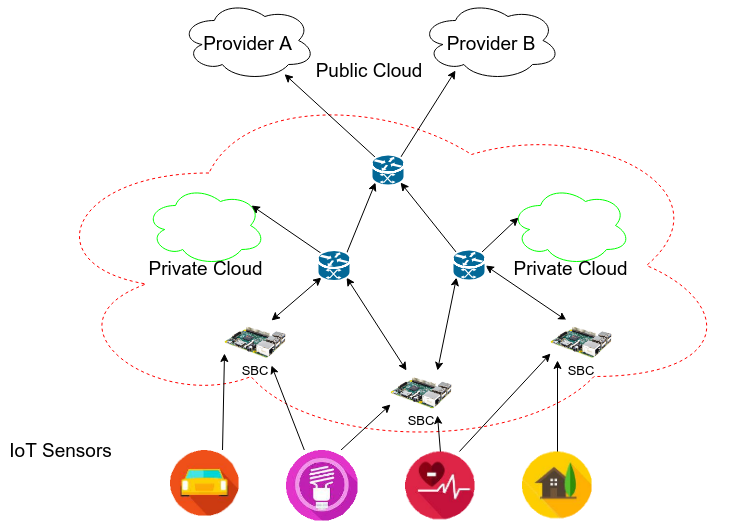
\includegraphics[width=1.0\linewidth]{figures/cassalesimgs-000.png}
      \caption{IDSA-IoT physical architecture and deployment scenario overview
      from \cite{Cassales2019a}.}
      \label{fig:mfog-phy-arch-cloud}
    \end{subfigure}
    \begin{subfigure}{.5\textwidth}
      \centerline{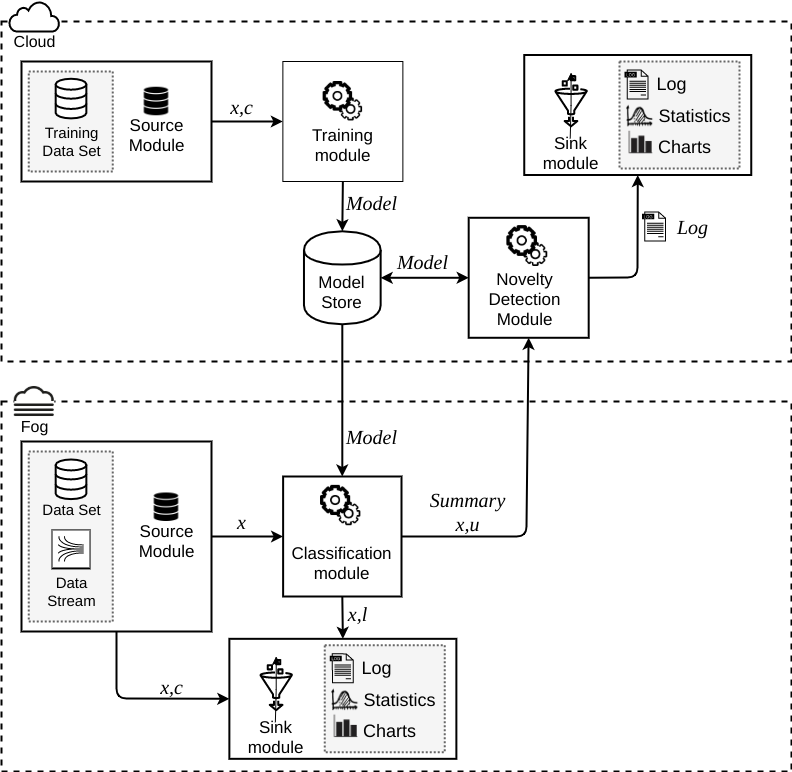
\includegraphics[width=0.95\linewidth]{figures/mfog-arch-v2_en.png}}
      \caption{\mfog components and communications overview, }
      \label{fig:mfog-architecture}
    \end{subfigure}
  }
  \caption{Architecture overview.}
  \label{fig:arch-overview}
\end{figure*}

%   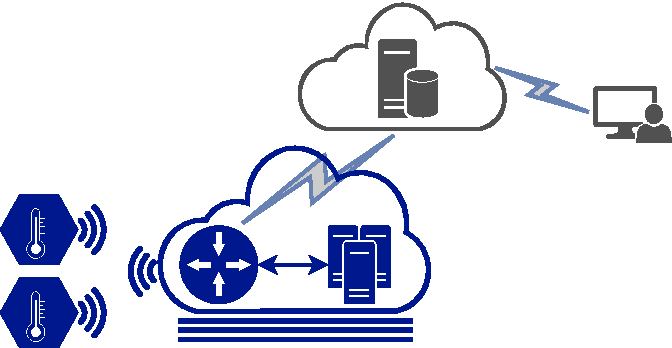
\includegraphics[width=0.9\linewidth,page=1]{figures/mfog-arch-fisica.svg.pdf}
% The overall organization of components, connections and interactions with external
% actors is shown in Figure \ref{fig:mfog-phy-arch-cloud},
% from bottom left to top right: sensor network; fog containing gateway router
% and novelty detection cluster; cloud storage for model, alarms and statistics
% and; human supervisor addressing alarms and statistics.

While our proposal focuses on fog computing resources, those resources are often limited
and they do not have the same reach and availability as traditional public cloud.
For that reason we also leverage the public cloud for model storage and distribution,
global novelty detection and alarm forwarding.

In Figure \ref{fig:mfog-architecture} we depict the overall architecture cut down to
individual modules:
three main functional modules being Training, Classification
and Novelty Detection handling MINAS main tasks;
and three auxiliary Source, Sink and Model Store, addressing external and internal connections
as well as providing facilities to our tests and experiments.

% enumerar módulos e funções
% \\descrever etapas do MINAS e onde se encaixa
% \\descrever onde módulos são multiplexados
% \\descrever casos de muiltiplos fluxos (redes locais)

% \todo{Needs review}
Source Module provides the input data stream for Offline and Online phases of MINAS
and is deployed in cloud and in fog for each respective phase and a variant for
testing on our experiments.
Model Store is another trivial module handling the initial Model storage and distribution
for Classification and Novelty Detection modules.
Last of the auxiliary modules is the Sink module, it denotes the consumer of labeling
output stream such as an alarm system, however in our implementation it is much more
complex, handling all tests metrics extraction and evaluations for our experiments,
aggregating all output (stream and logs) in files for proper analysis and later comparisons.
This module also differs in its software stack from the C language and MPI library,
for the ease of implementing such analysis needed by our experiments, 
courtesy of Pandas and NumPy libraries, we employed Python for this module.


Training Module encapsulates the Offline phase of MINAS and its output, being the
initial model, is stored by the Model Store.
Classification Module houses the homonymous task of MINAS Online phase and
is the focal point for parallelism in our proposal,
being replicated in the fog on each local network containing a cluster with one
or more nodes and each node multiple processes (limited to the individual CPU core count).
Novelty Detection Module can be also replicated,
one instance per local network and one global instance,
also handling the homonymous task of MINAS Online phase.
This modules takes as input all samples labeled with \emph{unknown},
stores them in a internal \emph{unknown} buffer and when this buffer is full,
triggers MINAS Novelty Detection task (clustering followed by validation).

% In Figure \ref{fig:mfog-architecture} we depict each logical component associated
% with each MINAS step and its communications, we also depict extra modules for sampling
% and measurements.
Each communication in Figure \ref{fig:mfog-architecture} shows the direction of the data flow
and identifies the data contained:
$Model$ is MINAS internal Model containing a set of cluster data structures,
$x,c$ identifies a sample with the real class,
$x$ is the sample without the real class,
$x,l$ identifies a sample with the assigned label,
$x,u$ is  sample with the \emph{unknown} label,
$summary$ is a statistical summary of model usage.

\subsection{Polices}\label{sec:polices}

The distribution of steps and tasks in various modules opens
data distribution and its impacts to discussion.
The decisions following these discussions can be organized in
several policies, some of them are:

\begin{itemize}
    \item Regarding the allocation of the Novelty Detection Module:
    \begin{itemize}
        \item At each fog node:
        patterns will be only detected if sufficient samples of them
        occur in the local observed network,
        use of the local node processing power and,
        a model synchronization mechanism must be added;
        \item In the cloud:
        detect patterns even when scattered on each local network,
        % also a model sharing mechanism
        % is not needed as the model has a single instance stored in the cloud,
        % the penalty of this choice is increased internet usage as any 
        each sample with \emph{unknown} label must be sent from edge to cloud implying 
        increased internet link usage and increased delay
        between the appearance of a pattern, its detection and its propagation
        to fog classifiers;
        \item On both:
        local \emph{unknown} buffer is maintained and novelty detection is local as well,
        once a sample is considered as noise or outlier it shall be sent to the cloud
        where the process repeats but with global data.
        This choice needs a more complex a model synchronization mechanism.
    \end{itemize}
    \item Regarding the model cleanup (forget mechanism):
    Even when a global novelty detection is used, local models can be optimized for faster
    classification using the its local model statistics, sorting last or removing clusters that
    are not in frequent use;
    \item Lastly, reclassification of \emph{unknowns}:
    In the novelty detection task in MINAS, the \emph{unknown} sample buffer is effectively
    classified using the new set of clusters, in 
    Algorithm \ref{alg:MINAS-nd} at line \ref{alg:MINAS-nd:reclassify} 
    % if the sample can be explained by a new cluster
    % it is removed from the \emph{unknown} sample buffer, however, this new labeling is not put forward
    the new cluster information also includes the set of samples composing that cluster,
    thus, if this new label assignment was put forth to the system output
    it would change the system data stream behavior from a 
    \emph{map} (meaning each input has one output)
    % , whereas if this feature was enabled the behavior would be
    to a \emph{flatMap} (each input can have many outputs)
    and introduce delayed outputs, more recent and perhaps more accurate.
\end{itemize}

% \begin{highlight}
% - Detecção de novidades e manutenção de modelo em ambiente distribuído:

%   - Mecanismo de ND local (síncrono) vs nuvem quanto à atraso de definição de modelo
%     (nesse ponto é onde a hipótese prevê maior diferença, grande ponto de interesse);

%   - Mecanismo de esquecimento local vs global (modelo único ou por nó);

%   - Atraso na reclassificação dos desconhecidos;
% \end{highlight}

\subsection{Implementation}\label{sec:implementation}

The original MINAS algorithm has a companion implementation (\refminas)
written in Java using MOA library base algorithms such as K-means and CluStream,
however in the new implementation only K-means is used.
% \refminas employs Java's double, a $64 bits$ number whose precision is not
% absolutely necessary and, as it is often necessary to shuffle between nodes via
% network and a small economy could be made with only a float number with $32 bits$.
Another difference between \refminas and \mfog is cluster radius calculation
from the distances of elements forming the cluster and the cluster's center,
where the former uses the maximum distance, the latter uses the standard deviation
of all distances as described in \cite{Faria2016minas}.

% Desafios de implementação:
% <!--
% - Definição de raio: desvio padrão das distâncias versus distancia máxima;
% - Atualização do micro-cluster limita-se à atualização do atributo \texttt{T};
% - Remoção de exemplos na implementação de referência é feita somente para o algoritmo \textit{CluStream};
% - Inclusão de borda: algoritmo inclui ($<=$), referência não inclui ($<$);
% - Seguiu-se as mesmas divergências anteriores para comparação dos resultados com a implementação referência;
% - Inclusão da borda;
% - Comportamento do mecânismo de \textit{sleep-model} não está definido, portanto não está ativo;
% - Processo de clusterização é limitado ao algoritmo \textit{K-Means}. Algoritmo \textit{CluStream} não está implementado;
% - -->
% - `Double vs Float`:
%   - Na implementação de referência, java double é utilizado;
%   - Na nova implementação duas versões foram testadas e a diferença de precisão entre as duas é de `5 E-8`;
%   - **Solução:** Use `float32` e economize os bits já que haverá comunicação entre nós e módulos;
% - Formato do fluxo de saída:
%   - Implementação de referência utiliza a tripla `(id, classe, etiqueta)`;
%   - Primeira implementação em C utiliza `(id, clusterLabel, clusterId, clusterRadius, label, distance, secondDistance)`;
%   - Segunda implementação utiliza dupla `(id, label)`;
%   - Na etapa de avaliação, independente de versão, o fluxo original é lido;
%   - **Solução:** O formato mínimo é `(id, label)`;

\newcommand{\val}{$\vec{v}\,$\xspace}
The stream format for input and output also of note.
Input information needed is the samples value (\val), this \val is a number
sequence of length $d$ (dimension).
In addition to the \val for evaluation and training purposes the class
identifier as single character, optionally an unique item identifier
(\emph{uid}) can be provided.
For output information and format the decision isn't so clear as we can't
predict future system integrations needs like only novelty alarms or every
samples original \val with assigned label so, we have a compromise and put only
enough information for the Sink Module (where the full information
from the testing file or stream can be accessed) meaning the format can be
defined as a tuple containing \emph{uid} and assigned label.

% - Reprocessamento dos exemplos utilizados para atualização do modelo:
%   - Muda o comportamento do operador de fluxo de `Map` para `Flatmap`, ou seja,
%     requer outro fluxo de saída para a transmissão de padrões novidade (alarmes);
%   - Para reclassificação a definição de raio é modificada de `r = f * σ` (fator
%     multiplicando desvio padrão) para `r = max(distance)` (distância máxima);
%   - Passível da crítica de *overfitting*. Isto é, este processo pode
%     inflar a métrica de precisão;
%   - **Solução:** *em aberto*;

Another implementation decision related to the output stream is whether or not
to reprocess, and add to the output stream, examples in the unknown buffer after
the novelty detection procedure, meaning one item can be classified once as
unknown and again with a label.
Our preliminary tests using this technique had increased true positives when compared to
not using it.
However this changes the stream operator behavior from a \textit{Map} to a
\textit{FlatMap} having duplicate entries on the output stream as previously
mentioned.
Regardless of choice the classification of the unknown buffer after a model
update, using the full model or just the added set of clusters, is done to
remove the examples ``consumed'' in the creation of a new cluster in the internals
of the clustering algorithm.
% This removal can be made less complex if using only new clusters 

% Próximos desafios:
% - Distribuição e paralelização para minimização de latência entre novo item no fluxo e sua classificação:
%   - Tempo de passagem da instância pelo classificador;
%   - Volume máximo do sistema;
%   - Diferenças de precisão de acordo com a carga;

For \mfog the Message Passing Interface (MPI, from \emph{Open MPI 4.0.4}) library was used.
In MPI programming, multiple processes of the same program are created by the
run-time and each process instance receives a rank parameter, for \mfog this
parameters indicate if the process is root, rank $0$, or leaf otherwise.
Beyond this division, each process also operates two threads, for the root
there is a sampler and detector threads, for the leafs each has a model receiver
thread and multiple classifier threads.
The overall sequence of interactions is shown in Figure \ref{fig:mfog-mpi-life}.

\begin{figure}[htb]
  \centerline{
    % 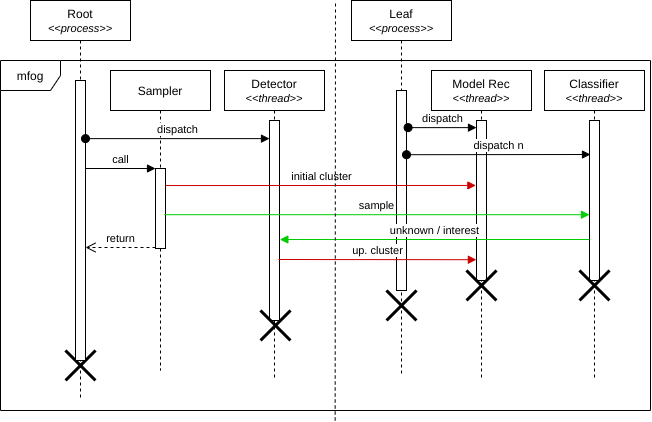
\includegraphics[width=0.7\textwidth]{figures/mfog-arch-mpi.png}
    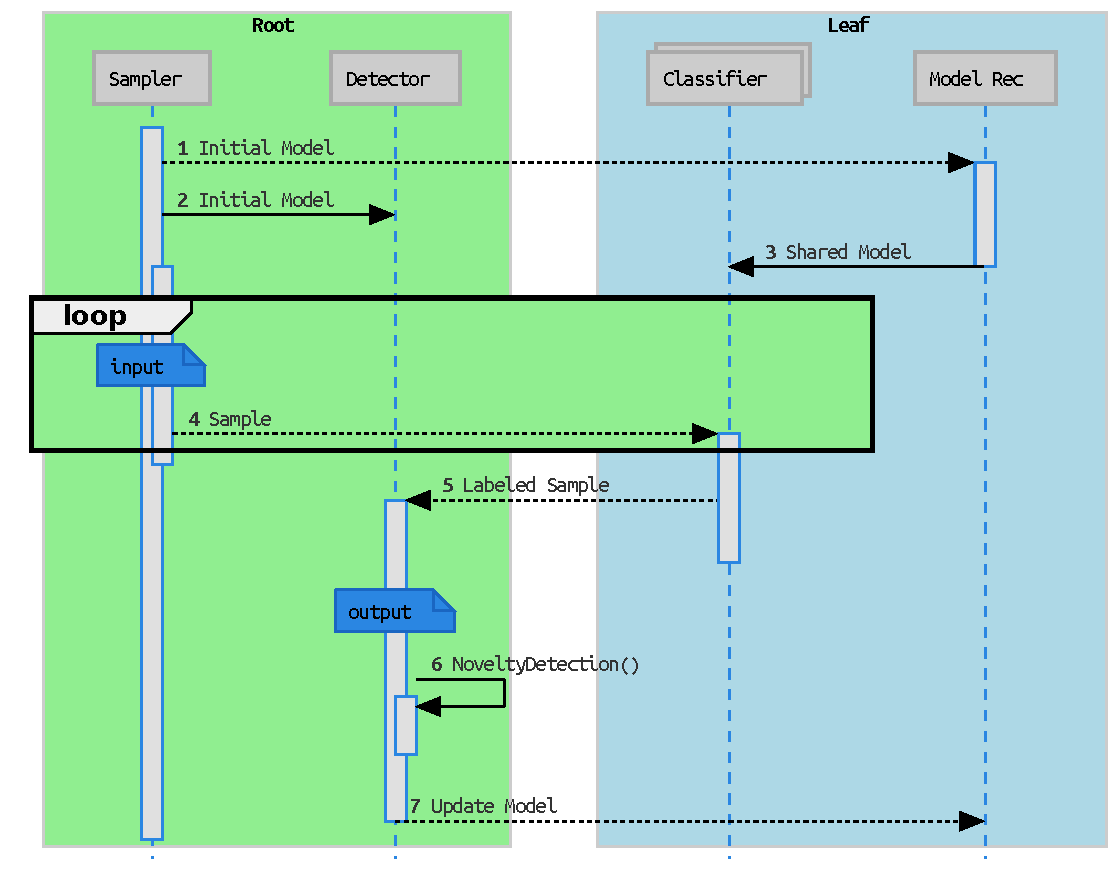
\includegraphics[width=\whencolumns{0.7}{1}\columnwidth,page=1]{figures/lifecycle.uml.svg.pdf}
    % \input{figures/lifecycle/lifecycle.latex}
  }
  \caption{\mfog life line overview.}
  \label{fig:mfog-mpi-life}
\end{figure}

The Sink Module was also build following reference techniques like
multi-class confusion matrix with label-class association
\cite{Faria2016minas}
to extract classification quality metrics.
